%!root = ../main.tex
\chapter{扩展问题的实证结果}\label{chap:4.1}
在基础回归的基础上,本文将在基准回归的基础上进行进一步的异质性分析,主要通过探讨两个问题:第一,地区之间的异质性效应是否仅限于与灾区的相对位置关系,还是也包括它们的绝对地理位置?第二,对于极端天气事件的反应是否仅与事件发生的相对时间有关,还是不同绝对时间点的反应也存在显著差异。本文将分别对这两个问题进行实证分析。

\section{地区异质性分析:适应性预期造成灾区结果差异}
在探讨极端天气事件对不同地区影响的差异性时,本文首先关注了地区对此类事件的反应是否存在显著的地域性差异。基于东部沿海地区频繁遭受降水事件的影响,居民可能因多次面对风险而逐渐形成了对此类风险的适应性预期。正如台风路径上的企业对自然灾害的反应效率提升\citep{0Do},频繁的降水可能为他们累积了经验,降低了对极端天气的敏感度\citep{陈思柳2021不同决策情境下的损失厌恶效应差异}。
相反,在干旱少雨的西部地区,由于降水事件较为罕见,由于降水相对较少对极端降水风险的敏感度不足,这可能导致他们在面对极端天气时的反应与东部地区存在显著差异。

为了验证这一假设,本研究根据国家统计局的划分标准,将样本划分为东部、中部和西部三个地区,并分别进行了回归分析。回归结果如表\ref{tab:het_geo}所示,基本与表\ref{tab:did1}和表\ref{tab:did2}一致。东部和中部地区在遭受极端降水事件后,所有地区的保险金额均有显著增长;然而,在灾区,交互项系数为负,表明保险金额有所下降,而在近灾区,保险金额的增长更为显著。

\begin{sidewaystable}[htbp]
    \centering
    \caption{分地区回归结果}\label{tab:het_geo}
    
\begin{tabular}{@{\extracolsep{5pt}}lcccccc}
\\[-1.8ex]\hline
\hline \\[-1.8ex]
& \multicolumn{6}{c}{\textit{Dependent variable: log(Coverage)}} \
\cr \cline{2-7}
\\[-1.8ex] & \multicolumn{1}{c}{East} & \multicolumn{1}{c}{Middle} & \multicolumn{1}{c}{West} & \multicolumn{1}{c}{East} & \multicolumn{1}{c}{Middle} & \multicolumn{1}{c}{West}  \\
\\[-1.8ex] & (1) & (2) & (3) & (4) & (5) & (6) \\
\hline \\[-1.8ex]
 Disaster & -0.090$^{***}$ & 0.054$^{***}$ & -0.159$^{***}$ & & & \\
& (0.006) & (0.008) & (0.006) & & & \\
 Disaster:Post & -0.121$^{***}$ & -0.136$^{***}$ & 0.123$^{***}$ & & & \\
& (0.007) & (0.009) & (0.008) & & & \\
 Neighbor & & & & -0.233$^{***}$ & -0.136$^{***}$ & -0.490$^{***}$ \\
& & & & (0.016) & (0.018) & (0.129) \\
 Neighbor:Post & & & & 0.246$^{***}$ & 0.052$^{***}$ & 0.570$^{***}$ \\
& & & & (0.017) & (0.019) & (0.129) \\
 Post & 0.065$^{***}$ & 0.036$^{***}$ & -0.171$^{***}$ & 0.065$^{***}$ & 0.037$^{***}$ & -0.172$^{***}$ \\
& (0.004) & (0.004) & (0.004) & (0.004) & (0.004) & (0.004) \\
%  Prem\_before & 0.185$^{***}$ & 0.107$^{***}$ & 0.067$^{***}$ & 0.174$^{***}$ & 0.106$^{***}$ & 0.071$^{***}$ \\
% & (0.006) & (0.030) & (0.016) & (0.006) & (0.034) & (0.016) \\
%  log(GDP) & 0.000$^{}$ & 0.000$^{}$ & -0.000$^{}$ & 0.000$^{}$ & 0.000$^{}$ & -0.000$^{}$ \\
% & (0.000) & (0.000) & (0.000) & (0.000) & (0.000) & (0.000) \\
%  log(Penetration) & 0.906$^{***}$ & 0.029$^{***}$ & 0.071$^{***}$ & 0.909$^{***}$ & 0.027$^{***}$ & 0.116$^{***}$ \\
% & (0.005) & (0.007) & (0.005) & (0.005) & (0.008) & (0.005) \\
%  log(Price) & 0.312$^{***}$ & 0.684$^{***}$ & 0.848$^{***}$ & 0.296$^{***}$ & 0.672$^{***}$ & 0.852$^{***}$ \\
% & (0.001) & (0.002) & (0.001) & (0.001) & (0.002) & (0.002) \\
Intercept & 11.386$^{***}$ & 9.757$^{***}$ & 9.331$^{***}$ & 11.444$^{***}$ & 9.793$^{***}$ & 9.298$^{***}$ \\
& (0.005) & (0.006) & (0.007) & (0.006) & (0.007) & (0.007) \\
Controls & True & True & True & True & True & True \\
\hline \\[-1.8ex]
 Observations & 481063 & 123513 & 104695 & 450350 & 107232 & 96922 \\
 $R^2$ & 0.333 & 0.593 & 0.764 & 0.314 & 0.585 & 0.774 \\
 Adjusted $R^2$ & 0.333 & 0.592 & 0.764 & 0.314 & 0.585 & 0.774 \\
 Residual Std. Error & 0.704  & 0.439  & 0.375  & 0.718  & 0.447  & 0.364  \\
 F Statistic & 34345.705$^{***}$  & 25654.772$^{***}$  & 48356.638$^{***}$  & 29449.242$^{***}$  & 21634.683$^{***}$  & 47450.879$^{***}$  \\
    Year FE & True & True & True & True & True & True \\
\hline
\hline \\[-1.8ex]
\textit{Note:} & \multicolumn{6}{r}{$^{*}$p$<$0.1; $^{**}$p$<$0.05; $^{***}$p$<$0.01} \\
\end{tabular}

\end{sidewaystable}

然而,在西部地区,极端降水事件对远灾区的影响不显著,近灾区的交互项显著性较低,而灾区的交互项系数则显著为正,这与东部和中部地区的情况形成了鲜明对比。原因可能有两方面:一方面由于西部地区极端降水事件虽然也是二十年一遇,但绝对值相对较低,如图\ref{fig:rainings}所示,风险造成的损失相对有限,因此对居民行为的影响有限,导致远灾区和近灾区的显著性不高,同时回归的数值也相对较小。
另一方面,西部地区居民对极端降水风险的敏感度较低,容易低估了极端天气发生的概率\citep{tversky1973availability},导致保险覆盖不足。因此,在巨灾发生后,他们可能有补充保障的动机,这反映在灾区交互项系数显著为正上。

综上所述,本研究的结果揭示了不同地区对极端天气事件的反应确实存在显著的地域性差异。这种差异可能源于地区间对极端天气风险感知程度的不同,进而导致了不同的保险需求水平。但总的来说,这一发现与假设H\ref{hyp:1}的预期保持一致,即极端天气事件本质上是通过提高风险感知,导致家财险需求的增加

\begin{figure}[htbp]
    \centering
    \begin{minipage}{0.48\linewidth}
        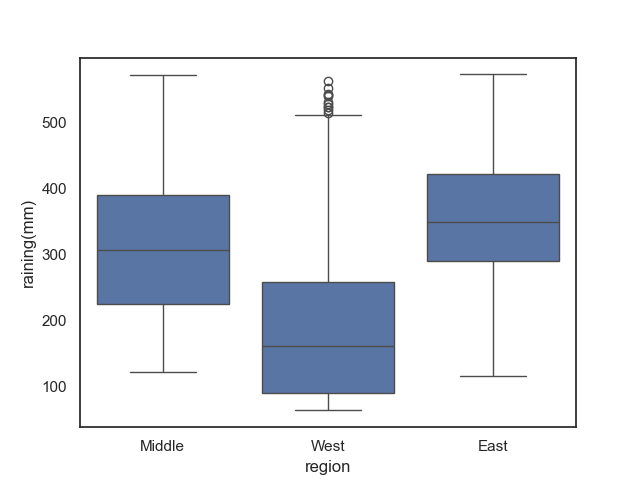
\includegraphics[width=\linewidth]{lib/img/rainings.png}
        \caption{样本中西部地区二十年一遇极端降水事件降水绝对值相对偏低}\label{fig:rainings}
    \end{minipage}
    \begin{minipage}{0.48\linewidth}
        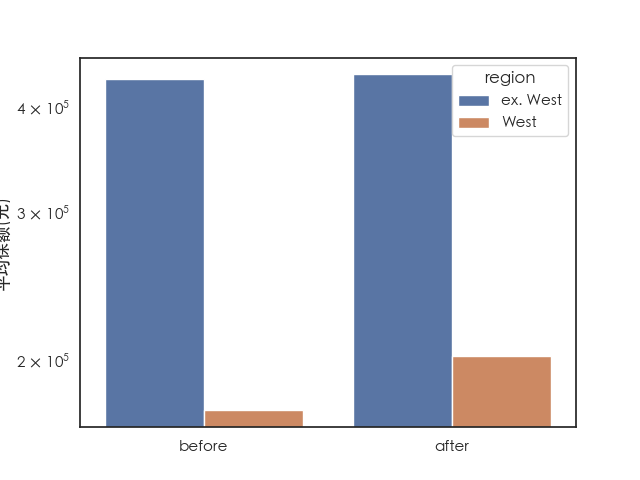
\includegraphics[width=\linewidth]{lib/img/covbyregion.png}
        \caption{西部地区在极端降水发生后有补充保险保障的动机}
    \end{minipage}
\end{figure}
\section{时间异质性分析:地震巨灾造成近灾区结果差异}
在探讨极端天气事件对不同时间点的反应差异时,本文以2008年为界,将样本最丰富的时间段分割为2003-2008年和2009-2013年两段,分别代表了两个不同的经济时期,得到的回归结果如表\ref{tab:het_time}所示,也与表\ref{tab:did1}和表\ref{tab:did2}基本一致,即表现为极端天气事件发生后控制组购买家财险的保额普遍提升,但灾区提升相对有限。

值得注意的是,近灾区交互项在2008年后显示出很强的正向提升,这可能是由于2008年汶川大地震使得居民对家庭所在周边的环境更为关注,对极端天气事件的风险感知提升,从而增加了对家财险的需求。这一发现也与假设H\ref{hyp:1}的预期一致,即极端天气事件通过提高风险感知从而增加家财险需求。
\begin{table}[htbp]
    \centering
    \caption{分时间回归结果}\label{tab:het_time}
    
\begin{tabular}{@{\extracolsep{5pt}}lcccc}
\\[-1.8ex]\hline
\hline \\[-1.8ex]
& \multicolumn{4}{c}{\textit{Dependent variable: log(Coverage)}} \
\cr \cline{2-5}
\\[-1.8ex] & \multicolumn{1}{c}{2003-2008} & \multicolumn{1}{c}{2009-2013} & \multicolumn{1}{c}{2003-2008} & \multicolumn{1}{c}{2009-2013}  \\
\\[-1.8ex] & (1) & (2) & (3) & (4) \\
\hline \\[-1.8ex]
 Disaster & 0.017$^{*}$ & -0.013$^{}$ & & \\
& (0.010) & (0.014) & & \\
 Disaster:Post & -0.170$^{***}$ & -0.089$^{***}$ & & \\
& (0.012) & (0.017) & & \\
 Intercept & 11.821$^{***}$ & 12.417$^{***}$ & 11.859$^{***}$ & 12.542$^{***}$ \\
& (0.006) & (0.006) & (0.005) & (0.007) \\
 Neighbor & & & 0.440$^{***}$ & -0.297$^{***}$ \\
& & & (0.012) & (0.043) \\
 Neighbor:Post & & & 0.032$^{*}$ & 0.211$^{***}$ \\
& & & (0.014) & (0.045) \\
 Post & 0.072$^{***}$ & 0.087$^{***}$ & 0.086$^{***}$ & 0.033$^{***}$ \\
& (0.006) & (0.007) & (0.006) & (0.008) \\
%  Prem\_before & 0.196$^{***}$ & 0.784$^{***}$ & 0.336$^{***}$ & 0.768$^{***}$ \\
% & (0.011) & (0.011) & (0.010) & (0.012) \\
%  Price & 0.187$^{***}$ & 0.113$^{***}$ & 0.166$^{***}$ & 0.125$^{***}$ \\
% & (0.001) & (0.001) & (0.001) & (0.001) \\
\hline \\[-1.8ex]
 Observations & 268828 & 191588 & 301508 & 139476 \\
 $R^2$ & 0.102 & 0.156 & 0.119 & 0.183 \\
 Adjusted $R^2$ & 0.102 & 0.156 & 0.119 & 0.183 \\
 Residual Std. Error & 0.982  & 1.058  & 0.998  & 1.045  \\
 F Statistic & 6122.243$^{***}$  & 7057.294$^{***}$  & 8131.866$^{***}$  & 6243.412$^{***}$  \\
\hline
\hline \\[-1.8ex]
\textit{Note:} & \multicolumn{4}{r}{$^{*}$p$<$0.1; $^{**}$p$<$0.05; $^{***}$p$<$0.01} \\
\end{tabular}

\end{table}
